\documentclass{article}

\usepackage[shellescape]{gmp}
\usepackage[utf8]{inputenc}
\usepackage{german}

\usepackage{geometry}
\geometry{margin=2cm,tmargin=2.5cm,bmargin=2cm}

\usepackage{graphicx}
\DeclareGraphicsRule{*}{mps}{*}{}

\usepackage{pdflscape}

\usepackage{titling}
\setlength{\droptitle}{80px}

\usepackage{xcolor}
\definecolor{light-gray}{gray}{0.95}
\definecolor{gold}{HTML}{FFD700}
\definecolor{vared}{HTML}{BF0020}
\usepackage{nicefrac}

\usepackage{soul}

\usepackage[colorlinks=true,urlcolor=blue]{hyperref}

\usepackage{wrapfig}

\renewcommand{\figurename}{Abbildung}
\begin{document}
\title{\Large Einsendeaufgabe \\ Vorgehensmodelle}
\author{\normalsize Stefan Berger}
\date{}
\maketitle

\vspace{160px}

\pagebreak

\section{Scrum-Tool: Jira}
\paragraph{}
Da es bei meinem derzeitigen Arbeitgeber seit einigen Jahren intensiv genutzt wird und es mir zumindest aus der Sicht eines Softwareentwicklers sehr vertraut ist, habe ich Jira  als Scrum-Tool ausgewählt. Jira ist eine populäre Projektmanagementsoftware mit Spezialisierung auf Softwareentwicklung.

\begin{figure}[h]
  \centering
    \fcolorbox{gray}{white}{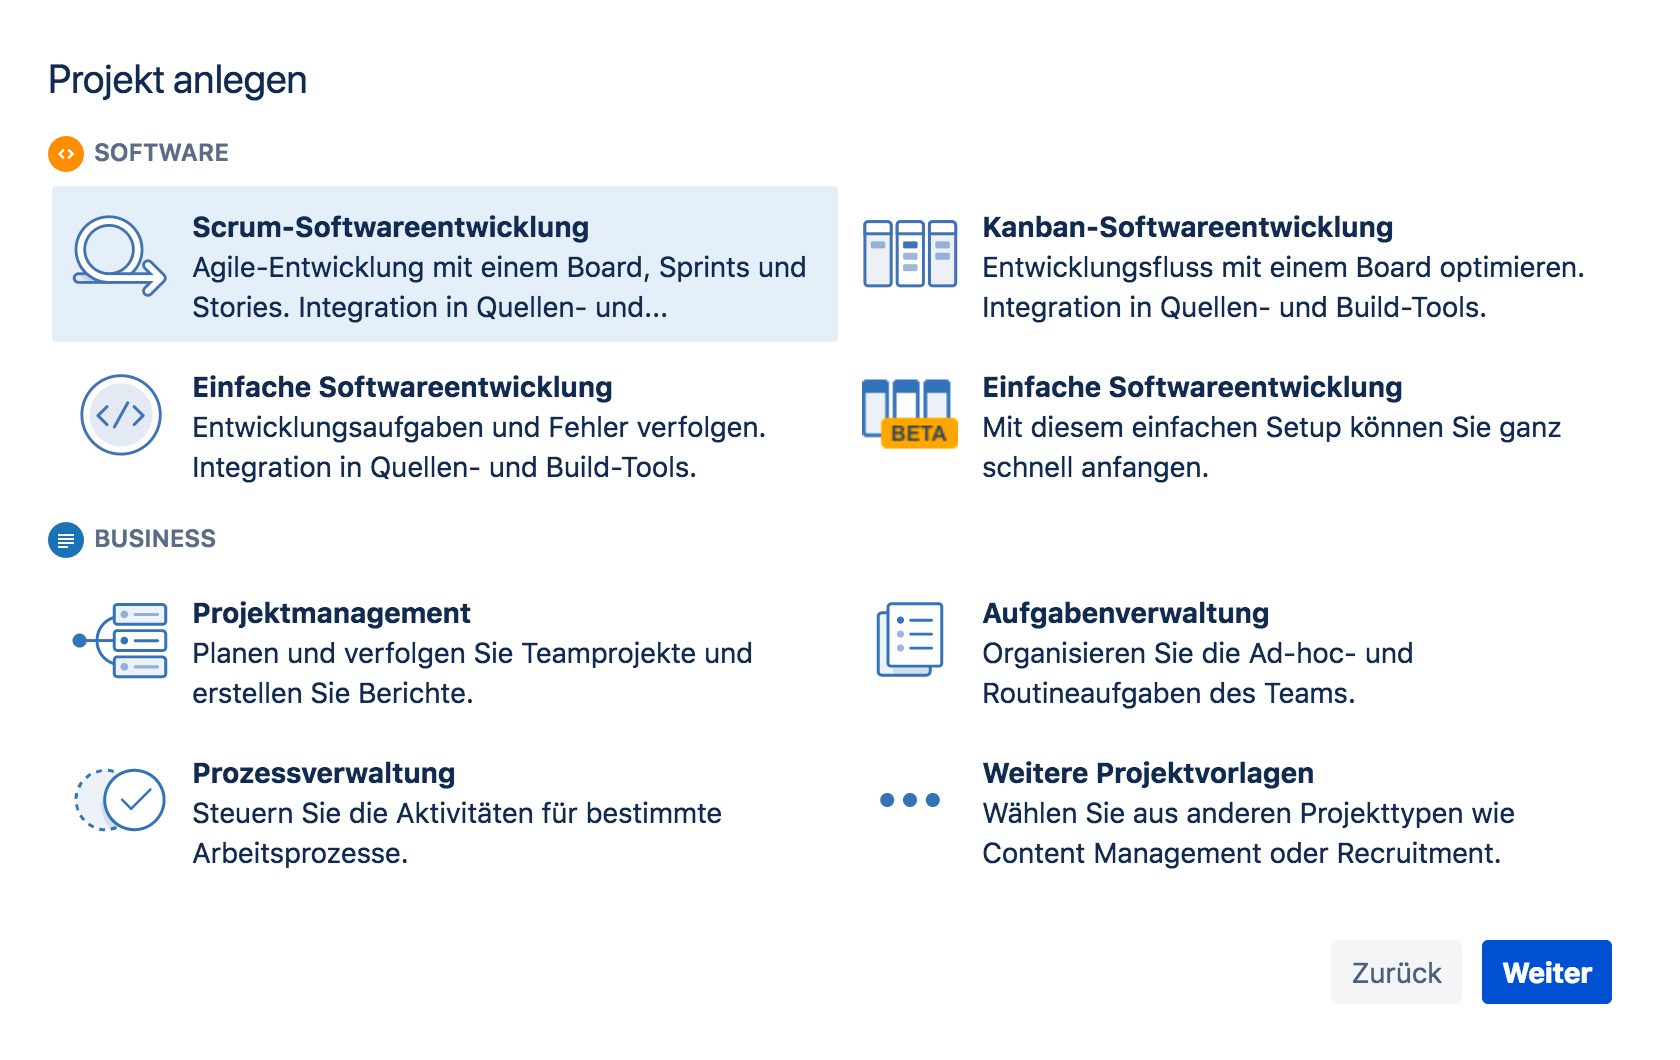
\includegraphics[scale=0.28]{psd/anlegen.png}}
  \label{assistent}
\end{figure}

\paragraph{}
Nachdem eine Projektart ausgewählt wurde kann ein Name angeben werden. Aus dem Namen wird automatisch ein Schlüssel generiert. Die User Stories, die anschließend erstellt werden, erhalten eine ID, die sich aus dem Schlüssel und einer fortlaufenden Nummer zusammensetzt.

\begin{figure}[h]
  \centering
  \fcolorbox{gray}{white}{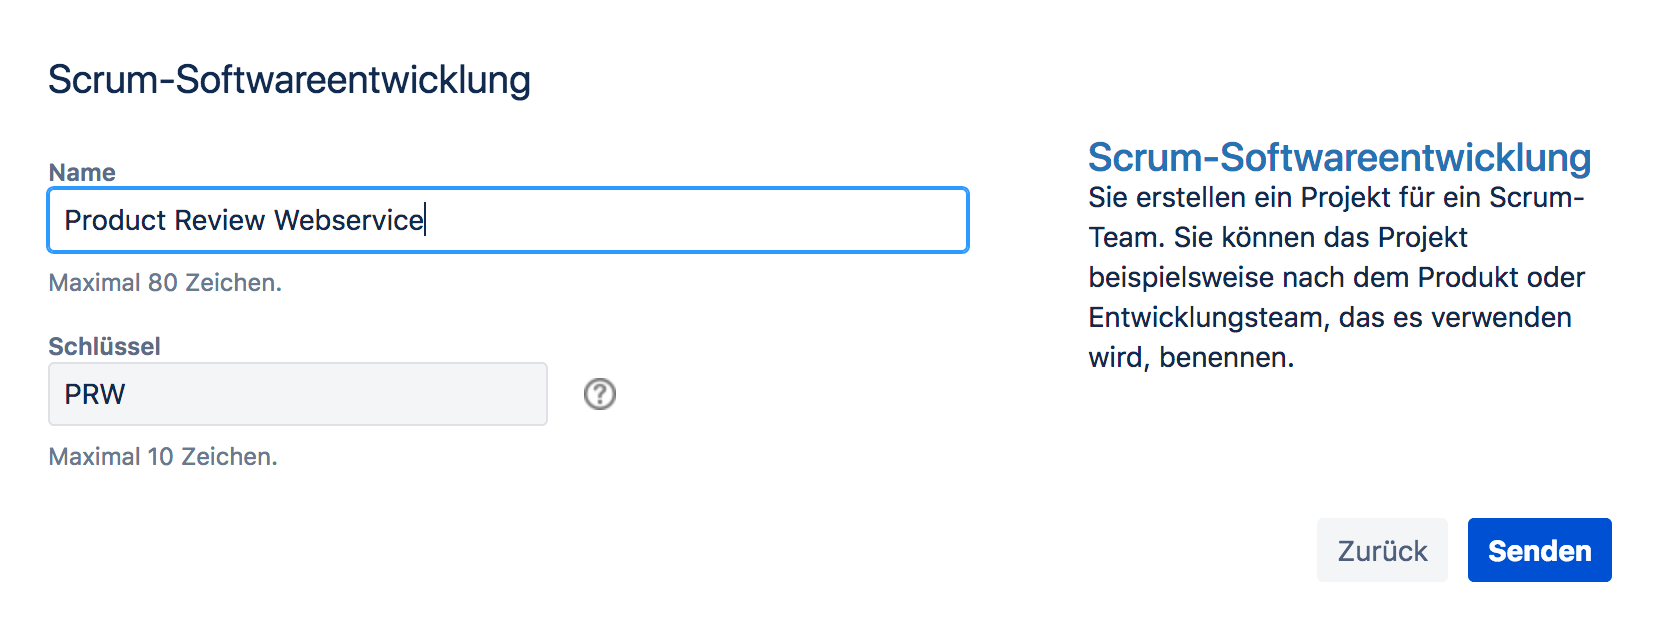
\includegraphics[scale=.28]{psd/pname.png}}
  \label{pname}
\end{figure}

\pagebreak

\section{Backlog}
\paragraph{}
Für das Projekt wird automatisch ein Backlog erstellt.

\begin{figure}[h]
  \centering
  \fcolorbox{gray}{white}{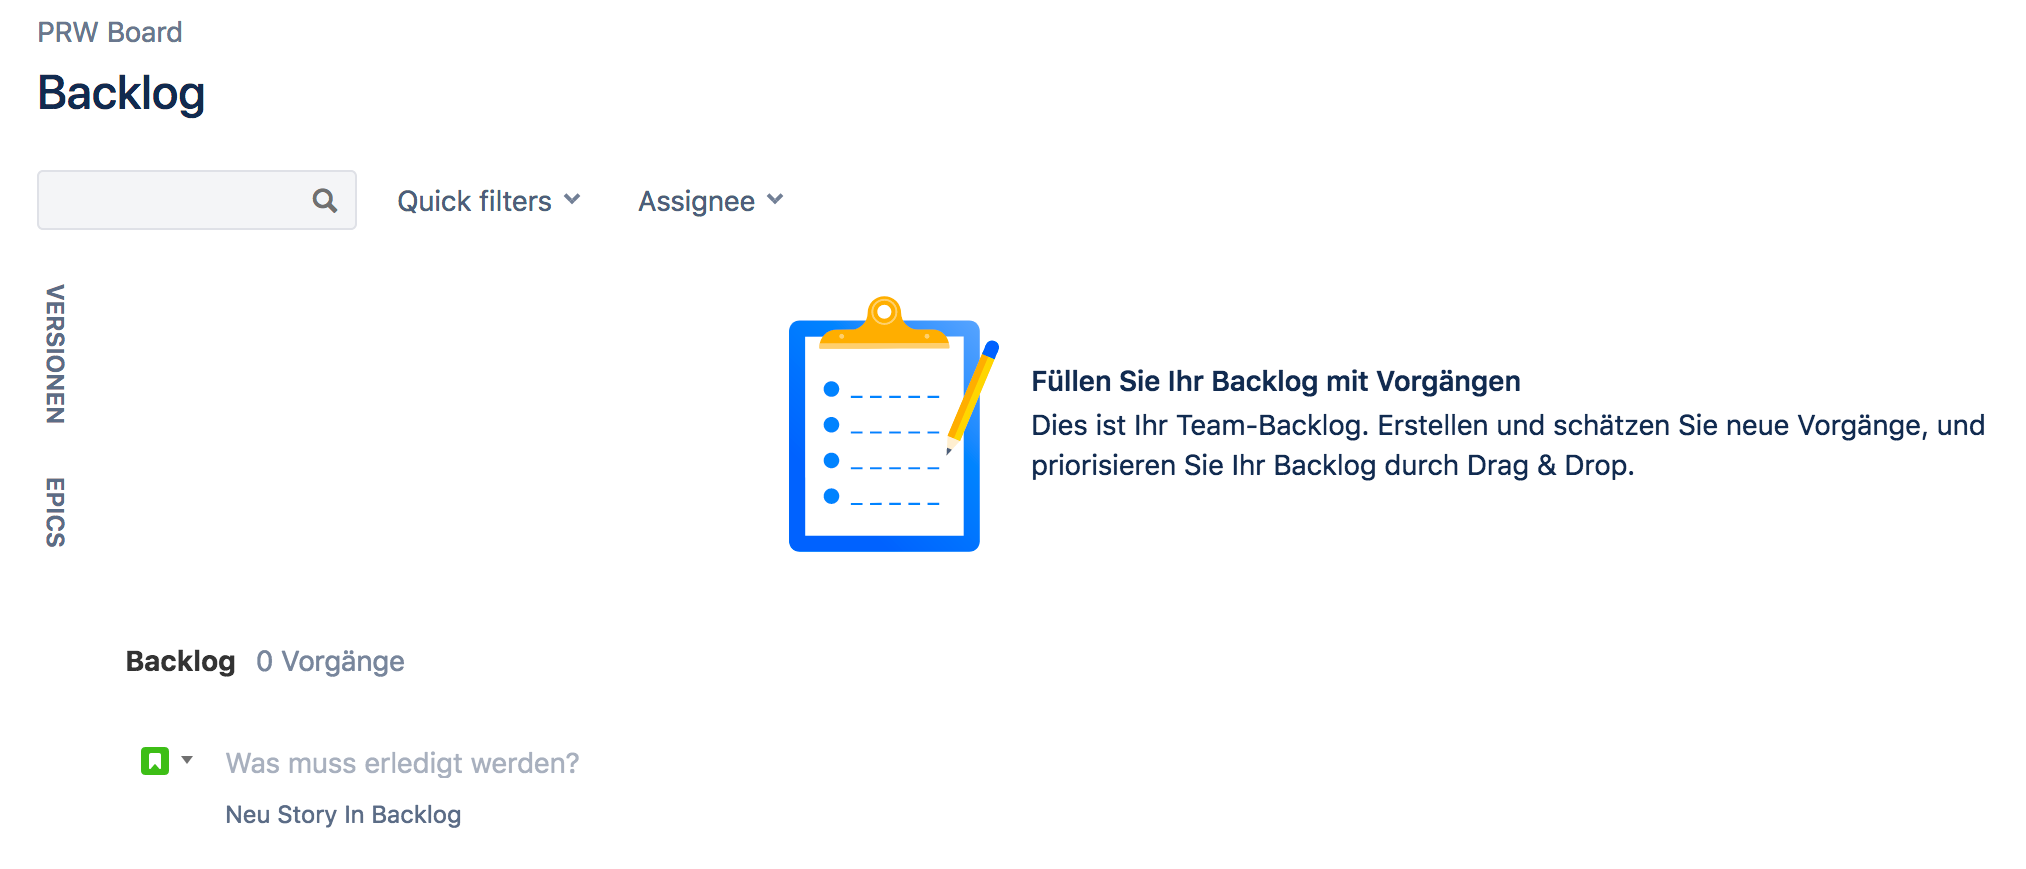
\includegraphics[scale=.2]{psd/backlog.png}}
  \label{backlog}
\end{figure}

\paragraph{}
Im Backlog können User Stories erstellt werden. Das geht sehr einfach; nach wenigen Minuten sind ausreichend viele Aufgaben für einen ganzen Sprint erstellt.

\paragraph{}
Die einzelnen Stories können vielseitig bearbeitet werden. Es gibt eine Markup-Language mit Überschriften und Tabellenformatierung, und es können Bilder wie zum Beispiel Screenshots in die Beschreibungen eingefügt werden. Besonders praktisch ist das Einfügen aus der Zwischenablage.

\begin{figure}[h]
  \centering
  \fcolorbox{gray}{white}{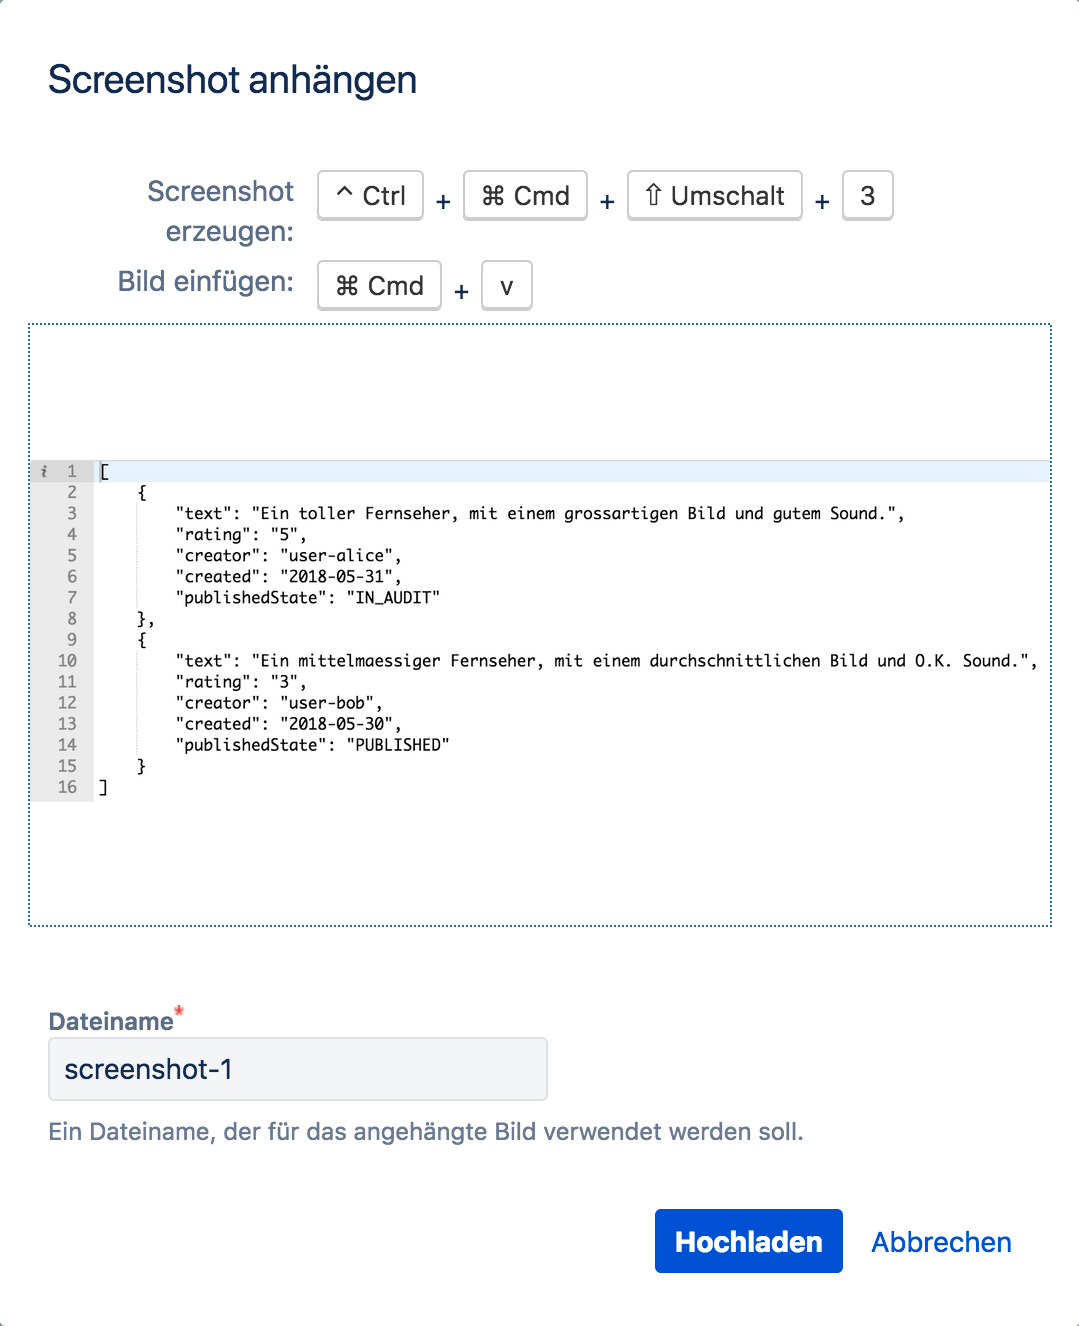
\includegraphics[scale=.23]{psd/clipboard.png}}
  \label{}
\end{figure}

\paragraph{}
So könnte eine fertig formulierte und formatierte User Story aussehen:

\begin{figure}[h]
  \centering
  \fcolorbox{gray}{white}{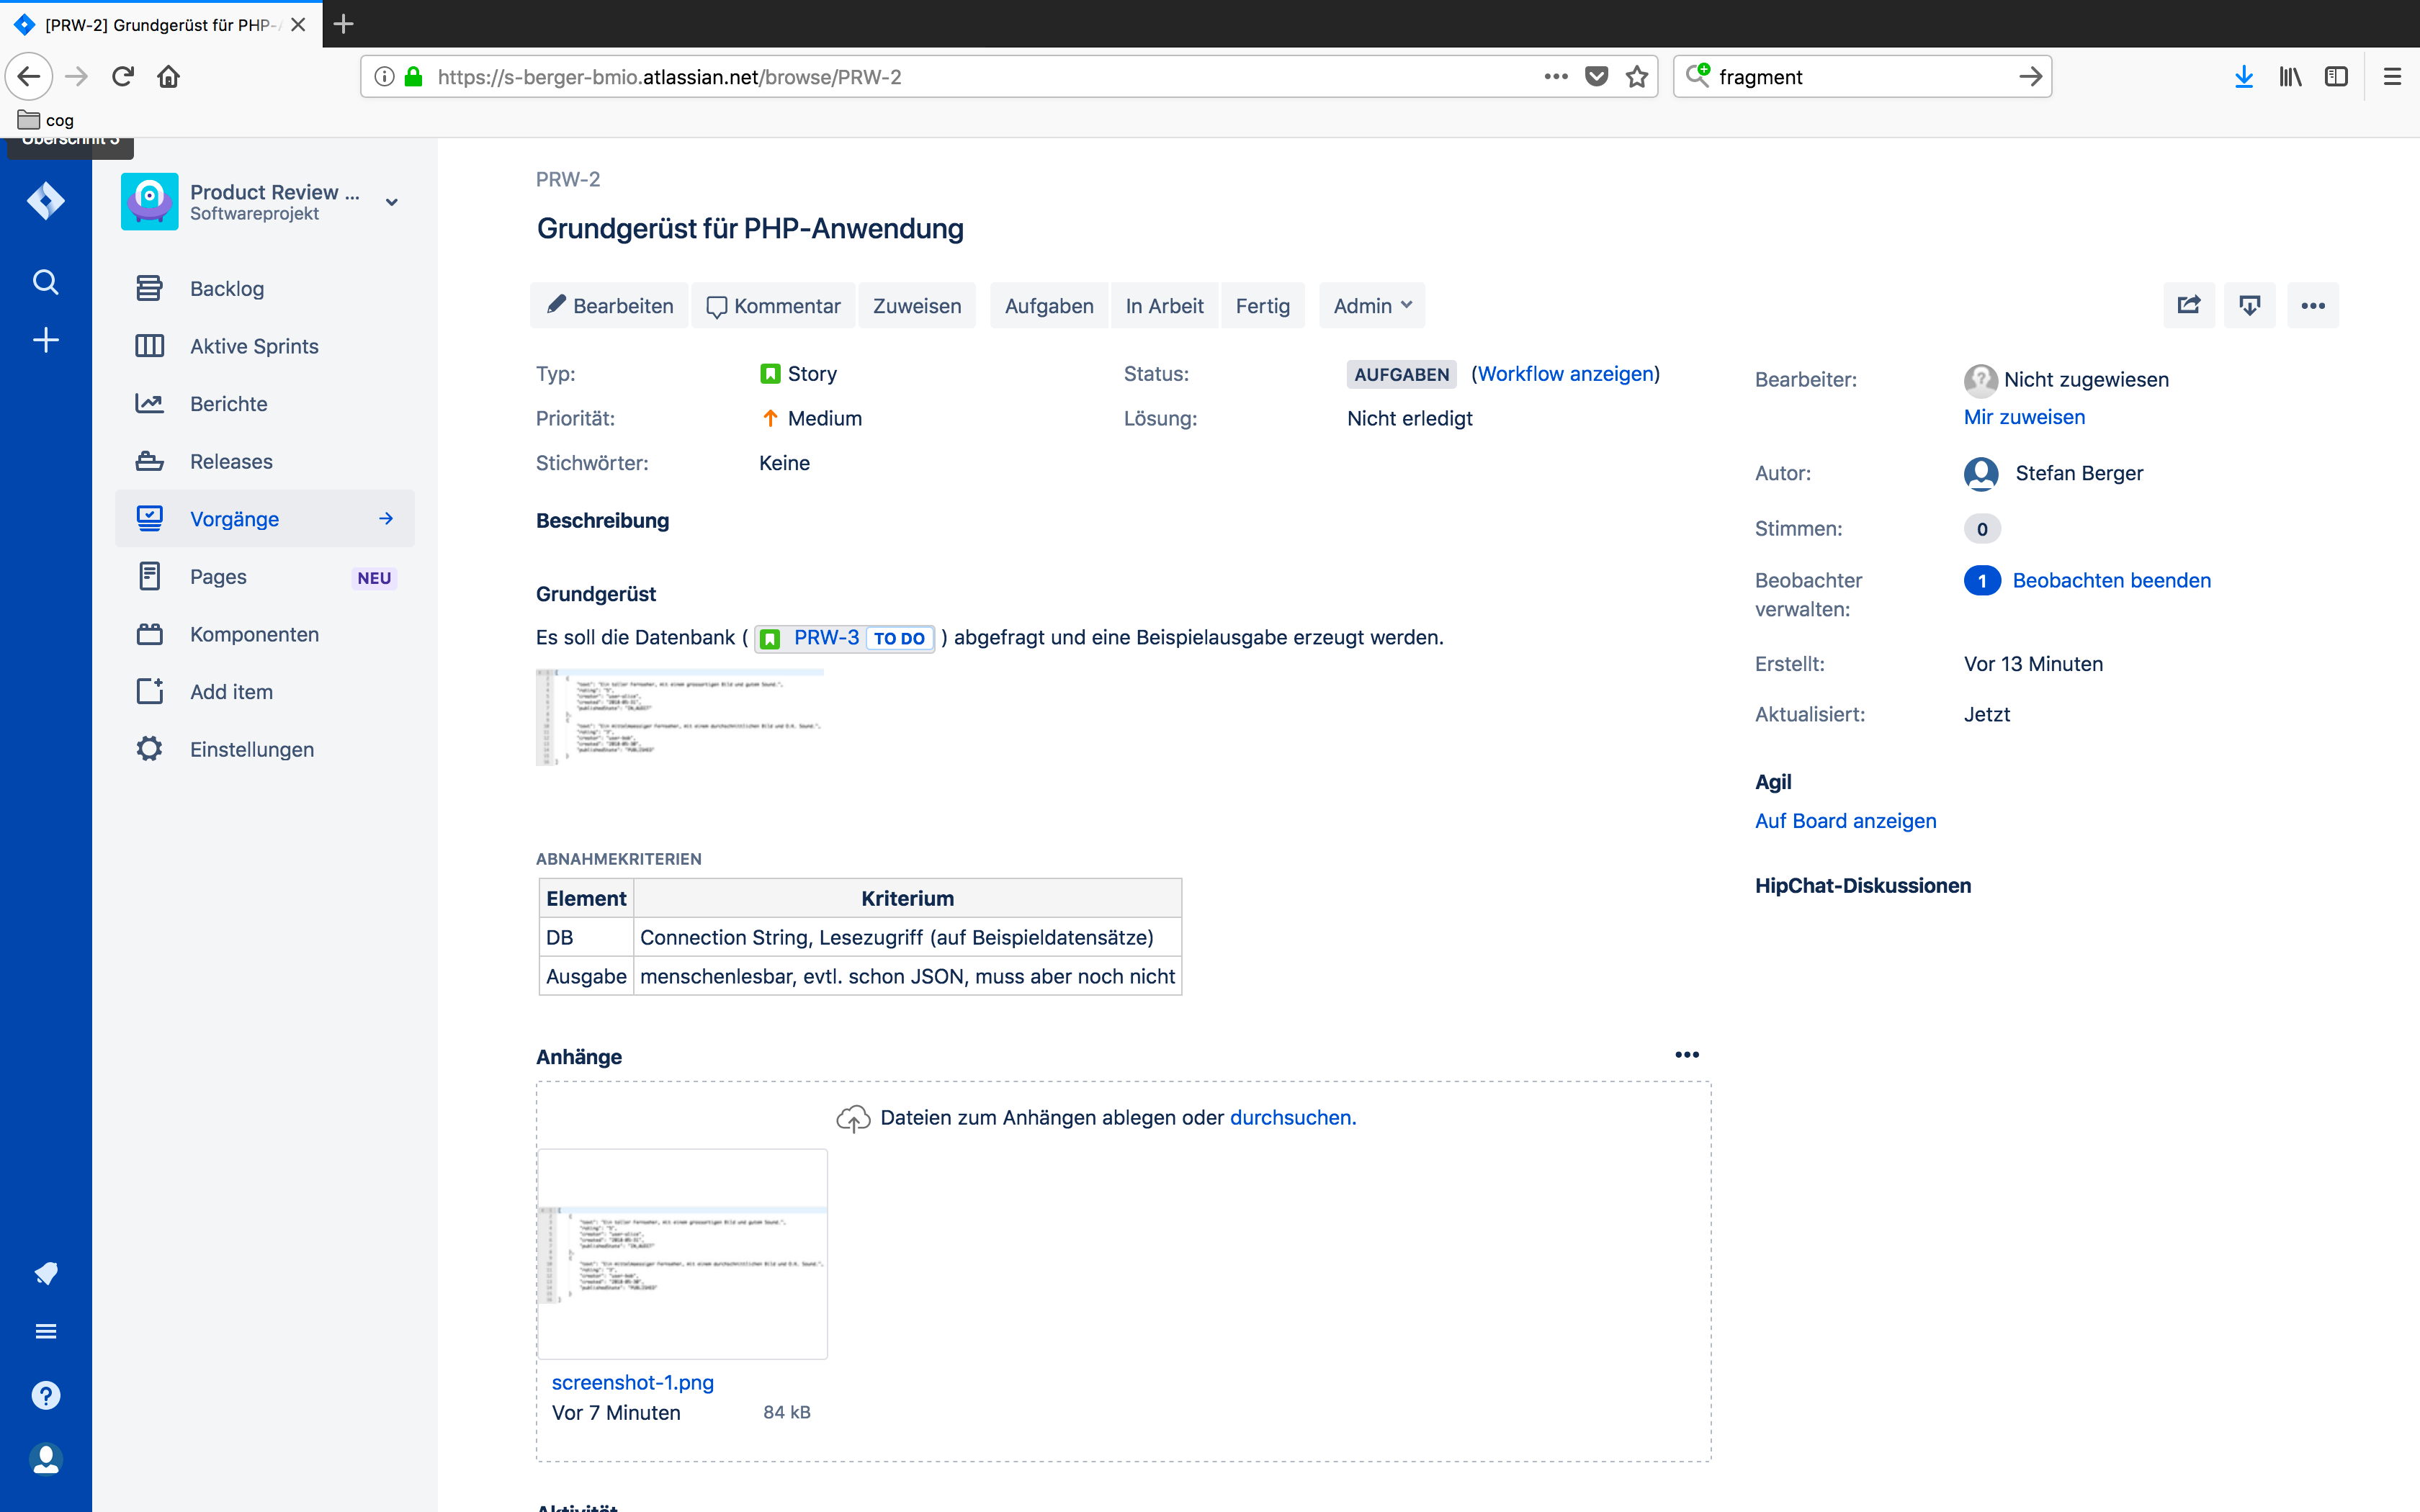
\includegraphics[scale=.15]{psd/ticket.png}}
  \label{}
\end{figure}

\paragraph{}
Die Einträge im Backlog können untereinander verknüpft werden. Kann beispielsweise eine Aufgabe erst angefangen werden, wenn eine andere erledigt ist, kann die User Story auf „blocked“ gesetzt werden.

\section{Sprint erstellen}
\paragraph{}
Sobald einige User Stories erstellt wurden bietet Jira an, einen Sprint zu erstellen.

\begin{figure}[h]
  \centering
  \fcolorbox{gray}{white}{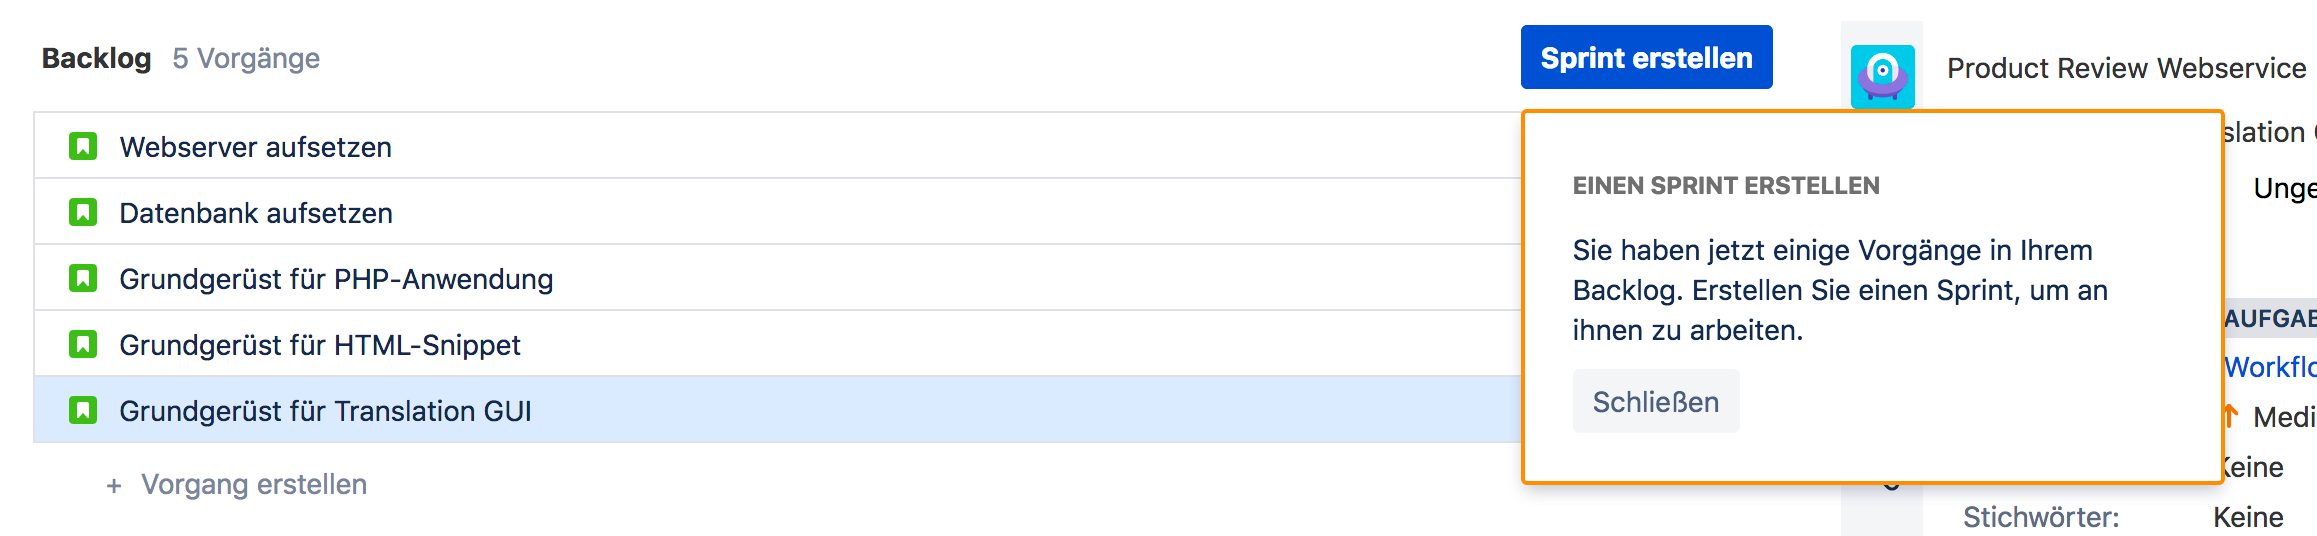
\includegraphics[scale=.2]{psd/create-sprint.png}}
  \label{}
\end{figure}

\paragraph{}
Die Vorgänge können danach dem neuen Sprint zugewiesen und der Sprint kann gestartet werden. Jira zeigt eine Warnmeldung an, wenn Stories noch nicht geschätzt wurden, d.h. eine Angabe zur Komplexität der Aufgaben fehlt. Die Schätzung wird normalerweise in Refinement-Meetings durch die Entwickler vorgenommen.

\paragraph{}
Der Sprint erhält einen Namen und ein Ziel. Anschließend wird mit der Bearbeitung der Stories begonnen.

\begin{figure}[h]
  \centering
  \fcolorbox{gray}{white}{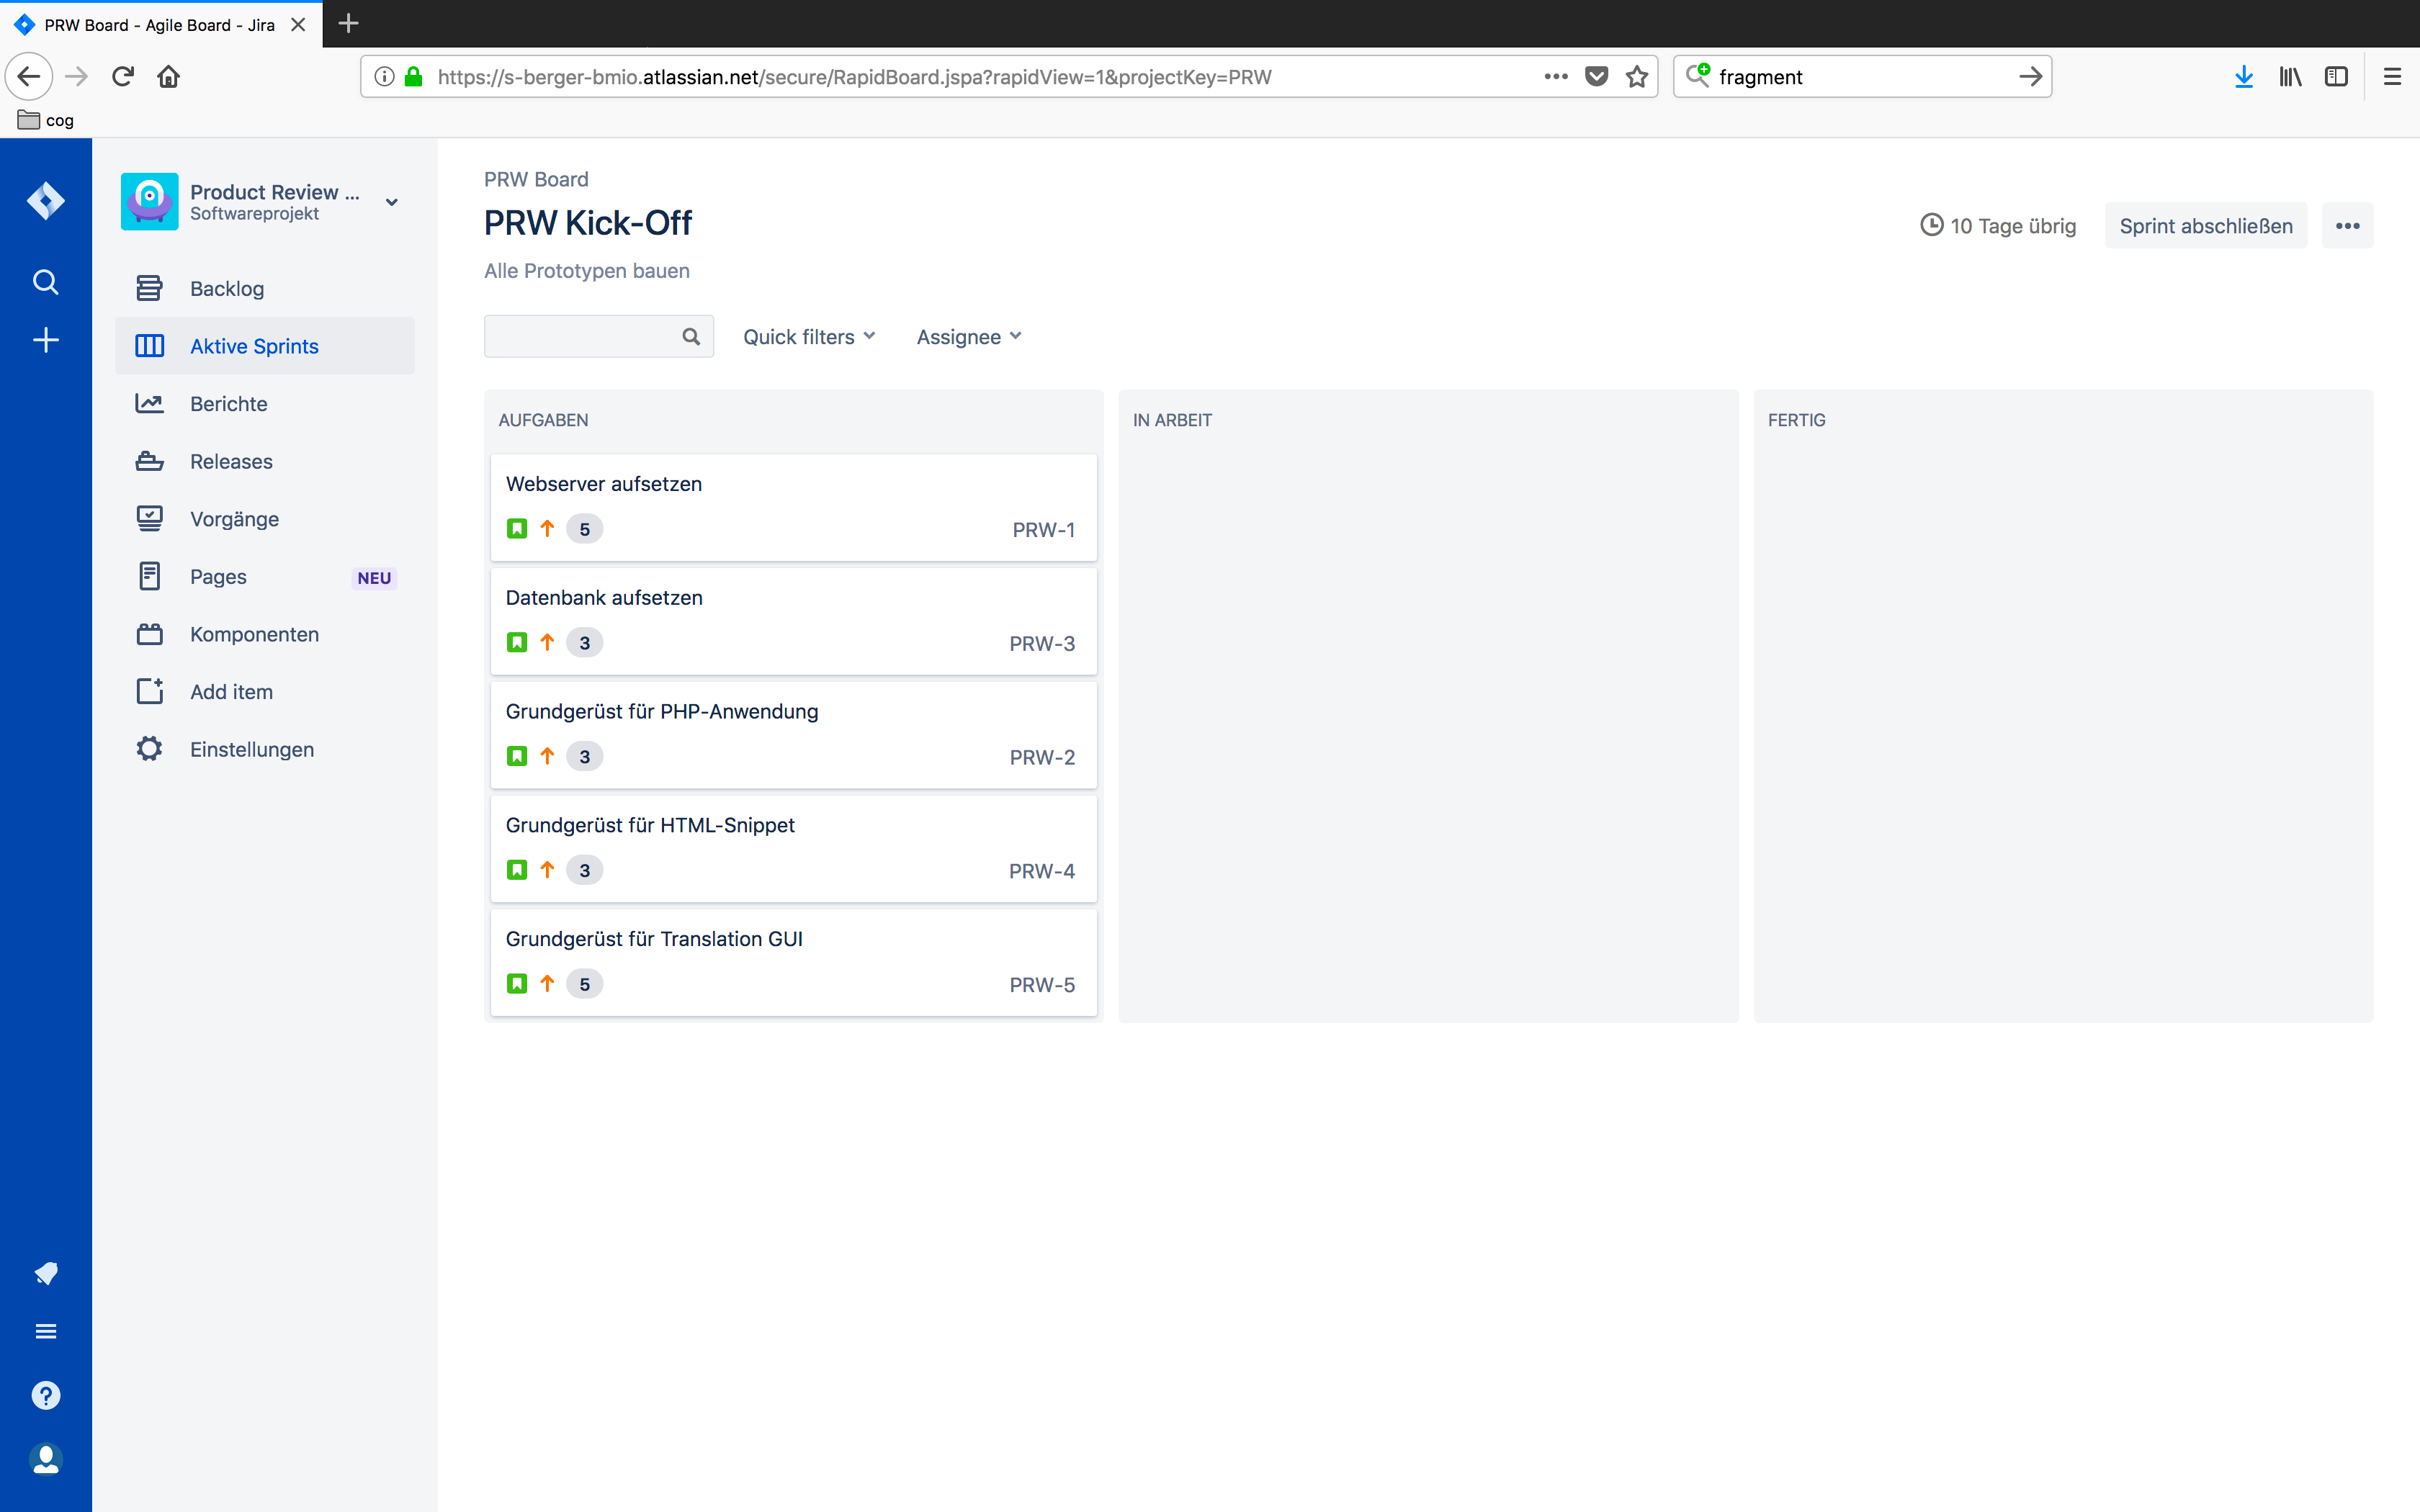
\includegraphics[scale=.13]{psd/sprint.png}}
  \label{}
\end{figure}

\section{Vorgänge bearbeiten}
\paragraph{}
Die Status der Stories können einzeln verändert werden. Jeder Story wird außerdem ein Bearbeiter zugewiesen. Auf diese Weise „ wandern“ die Vorgänge in den Spalten des Scrum-Boards von links nach rechts.

\begin{figure}[h]
  \centering
  \fcolorbox{gray}{white}{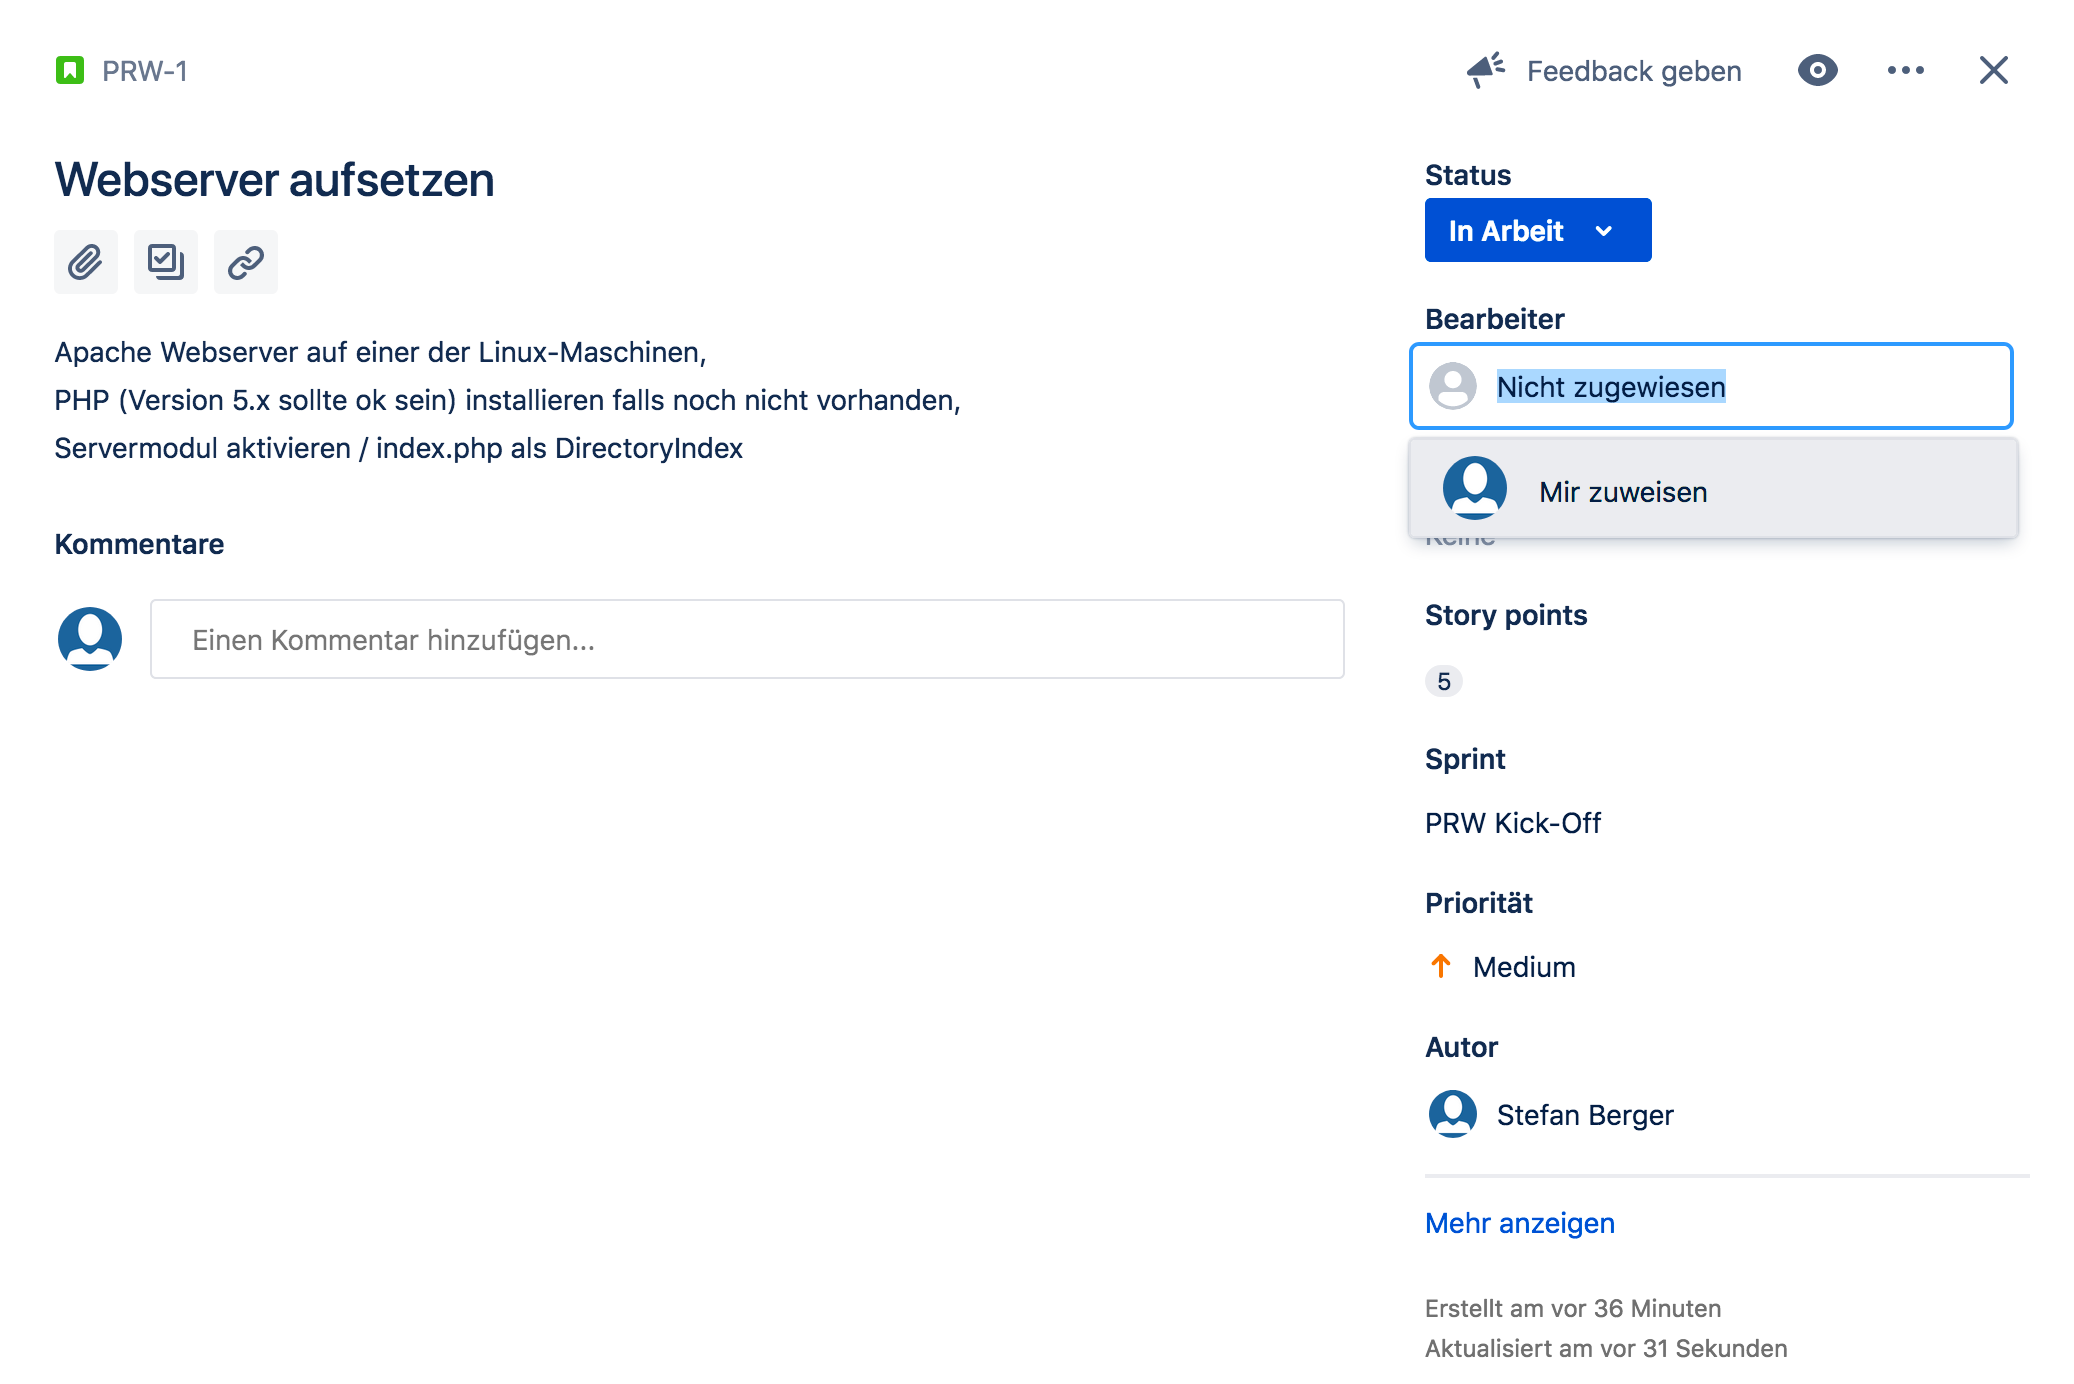
\includegraphics[scale=.15]{psd/assign.png}}
  \label{}
\end{figure}
\paragraph{}

\section{Sprint abschließen}
\paragraph{}
In diesem Beispiel war die Dauer des Sprints auf 2 Wochen, also zehn Arbeitstage, eingestellt. Am Ende dieser Zeitspanne, unabhängig davon wie viele der Stories bearbeitet wurden, wird der Sprint durch den Product Owner abgeschlossen. Jira zeigt daraufhin einen Sprint-Bericht an.

\begin{figure}[h]
  \centering
  \fcolorbox{gray}{white}{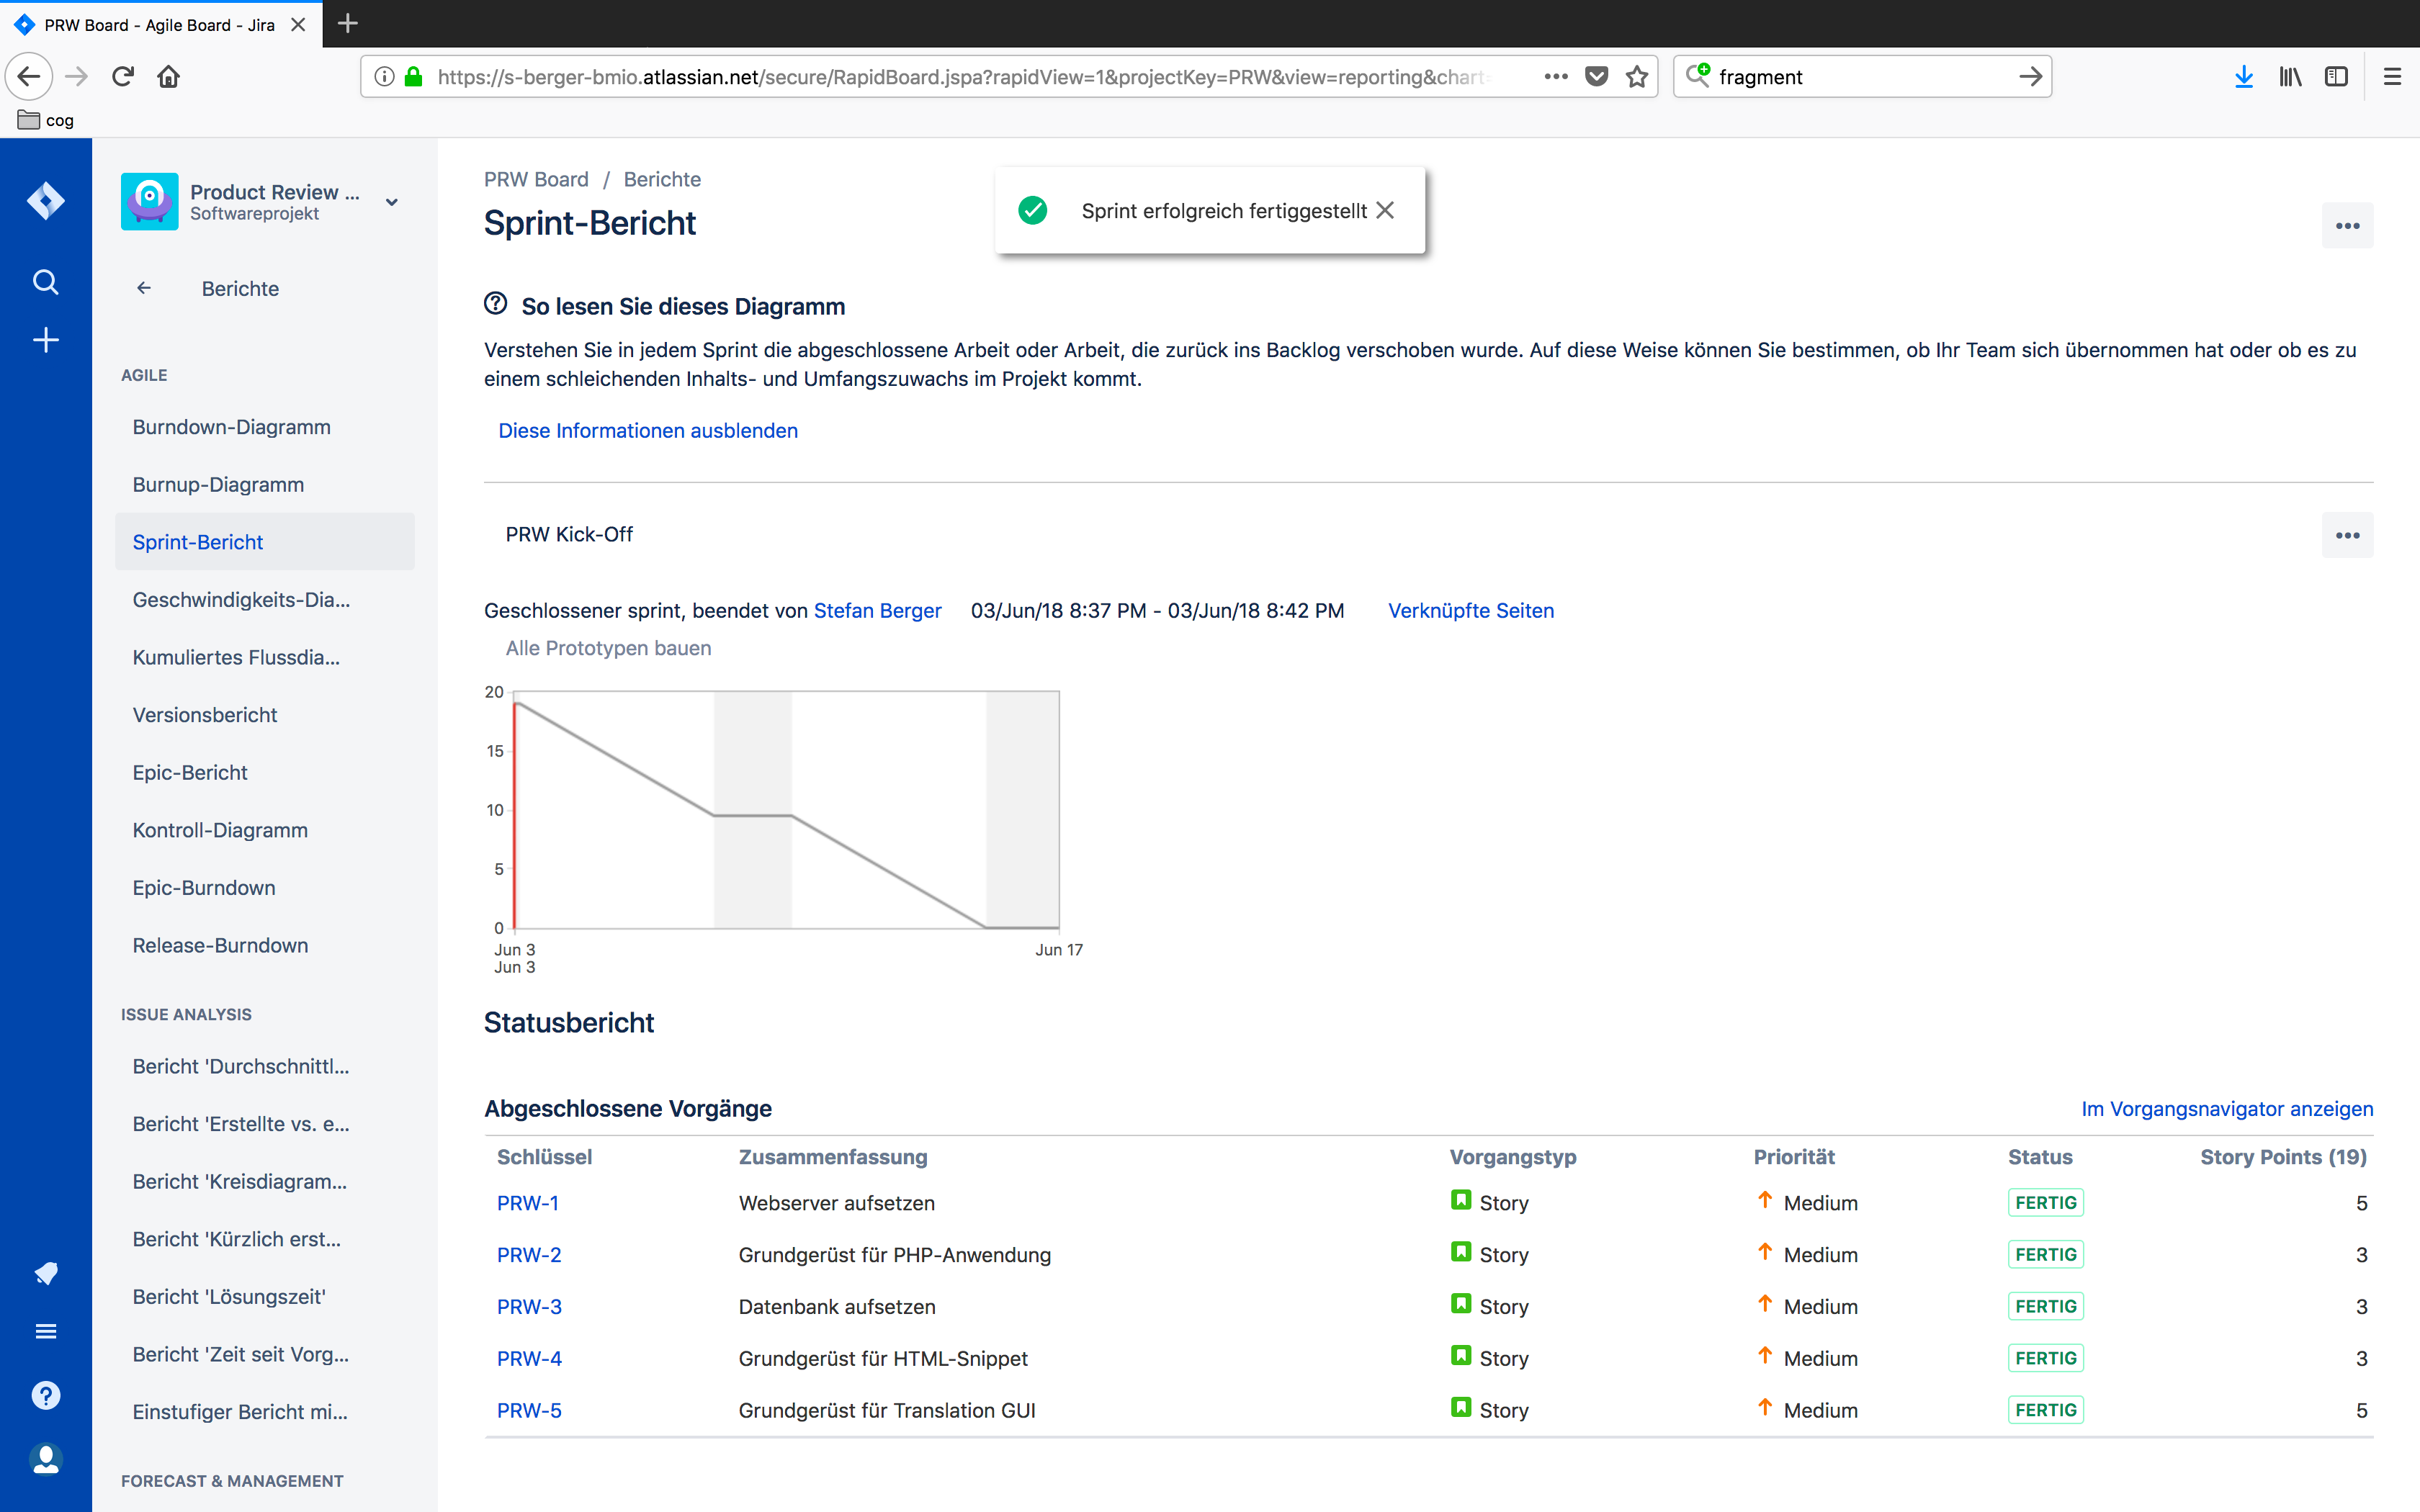
\includegraphics[scale=.15]{psd/report.png}}
  \label{}
\end{figure}

\end{document}
